%\subsection{Introductory Puzzle}

\begin{frame}
\begin{center}
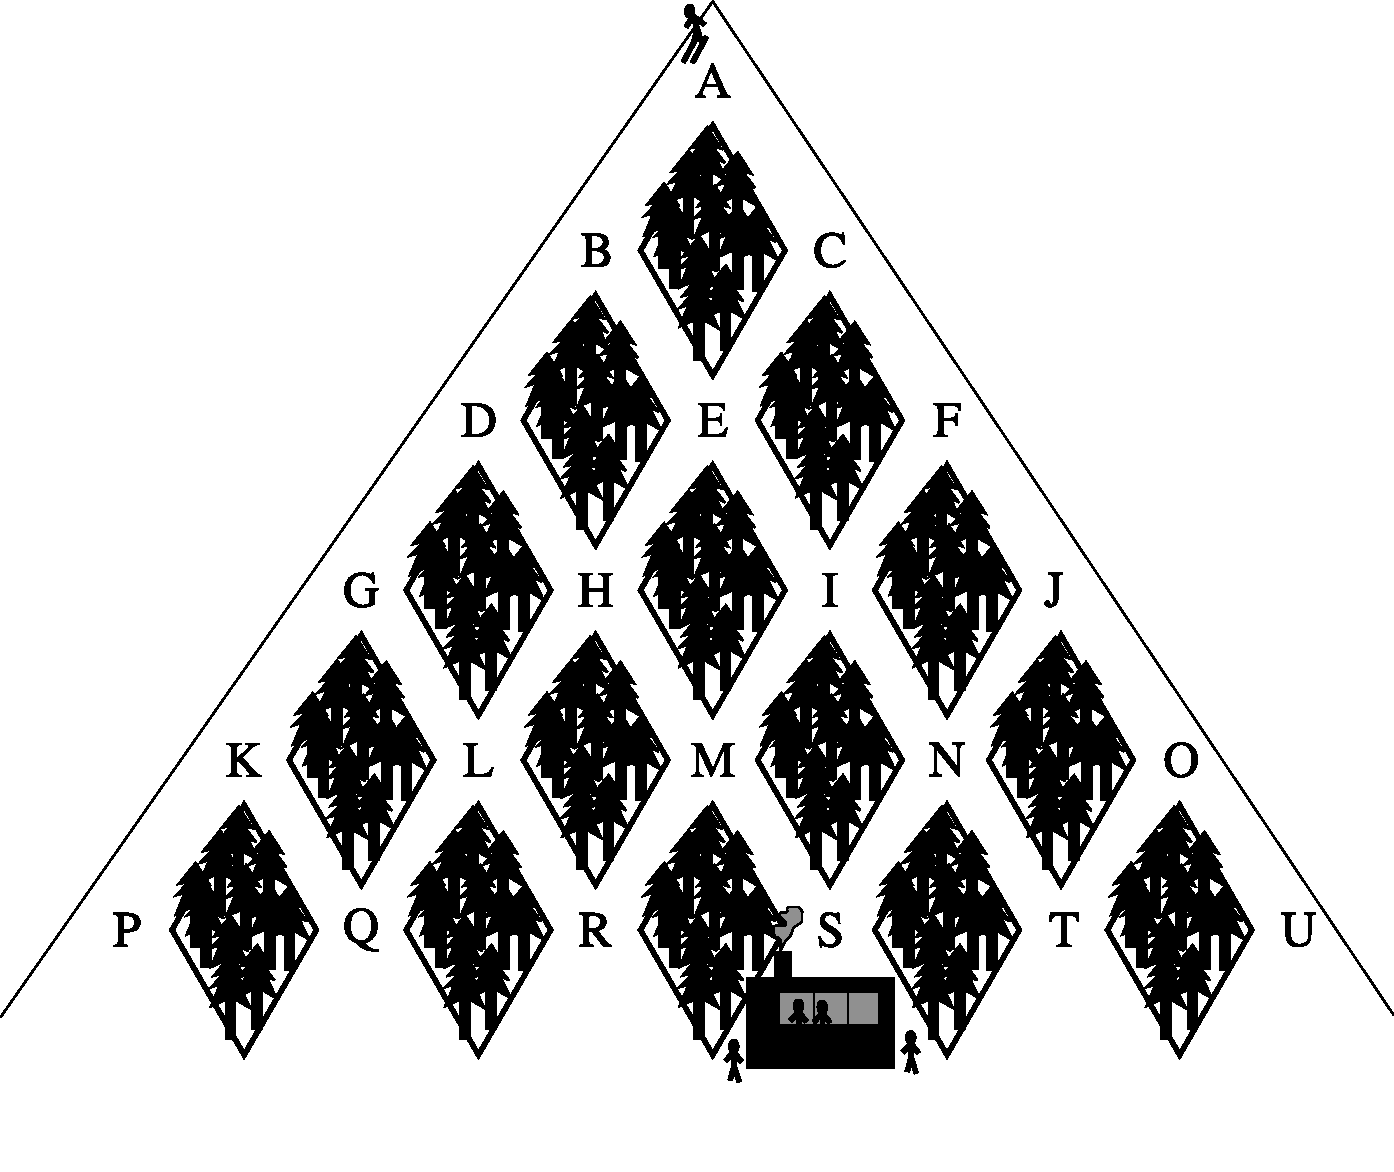
\includegraphics[scale=0.3]{3-4_binomial_distribution/figures/ski/ski.pdf}
\end{center}
Laney is at the top of the mountain (point A). She hopes to ski {\bf down} to point S (without going through trees or up hill). How many routes are possible?
\pause
\soln{\begin{center}
\fbox{10}
\end{center}}
\end{frame} 

\begin{frame}
\frametitle{Pascal's Triangle}
\begin{center}
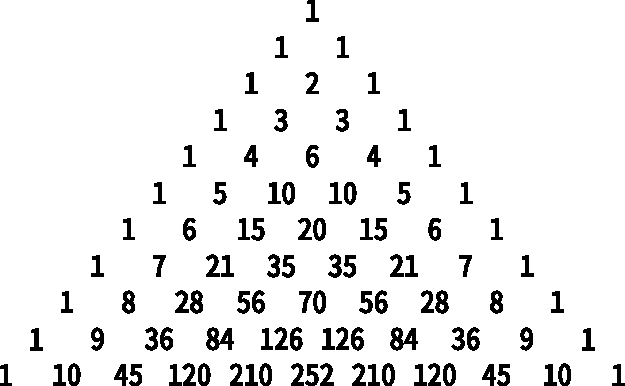
\includegraphics[scale=1]{3-4_binomial_distribution/figures/pascal/pascal.pdf}
\end{center}
\end{frame} 


\begin{frame}
Laney has 5 toes on her right foot. She wants to choose three  of these nails to paint green. How many different ways can Laney do this?
\begin{center}
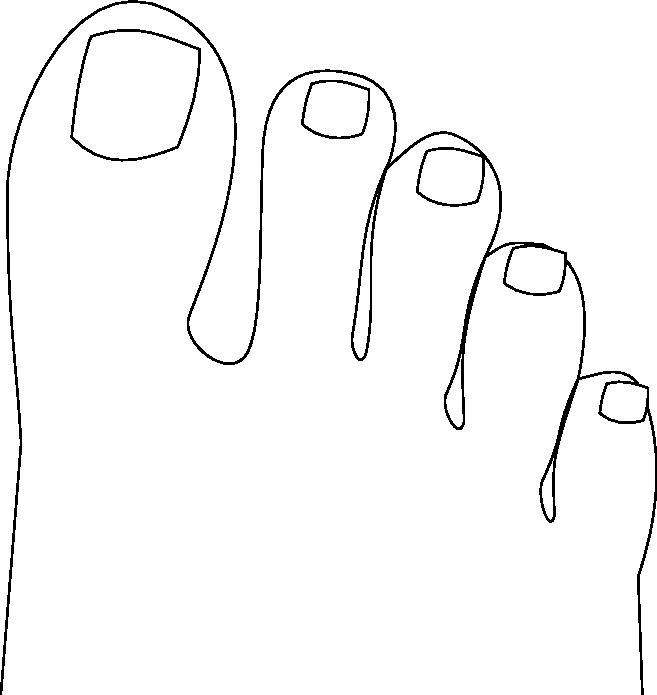
\includegraphics[scale=0.3]{3-4_binomial_distribution/figures/toes/toes.pdf}
\end{center}
\pause

\soln{
\begin{center}
\begin{tabular}{c c c c c}
GGGxx & GGxGx & GGxxG & GxGGx & GxGxG \\
GxxGG & xGGGx & xGGxG & xGxGG & xxGGG 
\end{tabular}
\end{center}
\begin{center}
\fbox{10}
\end{center}}

\end{frame} 


\begin{frame}
When given 7 dots, how many distinct line segments connect 2 of those dots? In other words, with 7 nodes, how many edges can be drawn?

\begin{figure}
    \begin{overprint}
    \onslide<1>\centering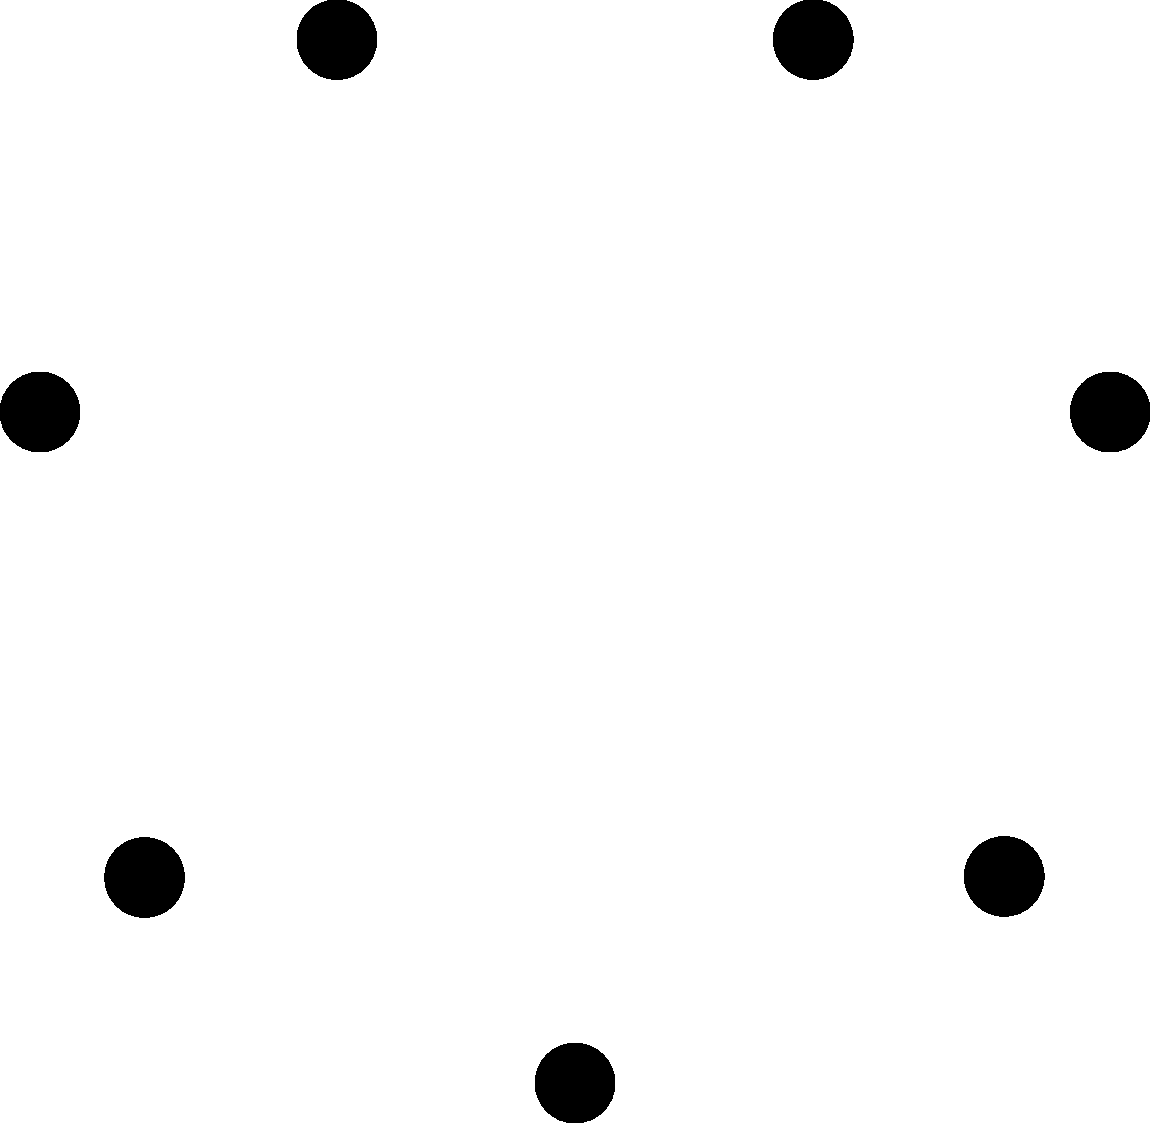
\includegraphics[scale=0.3]{3-4_binomial_distribution/figures/stars/dots_7.pdf}
    \onslide<2| handout:0>\centering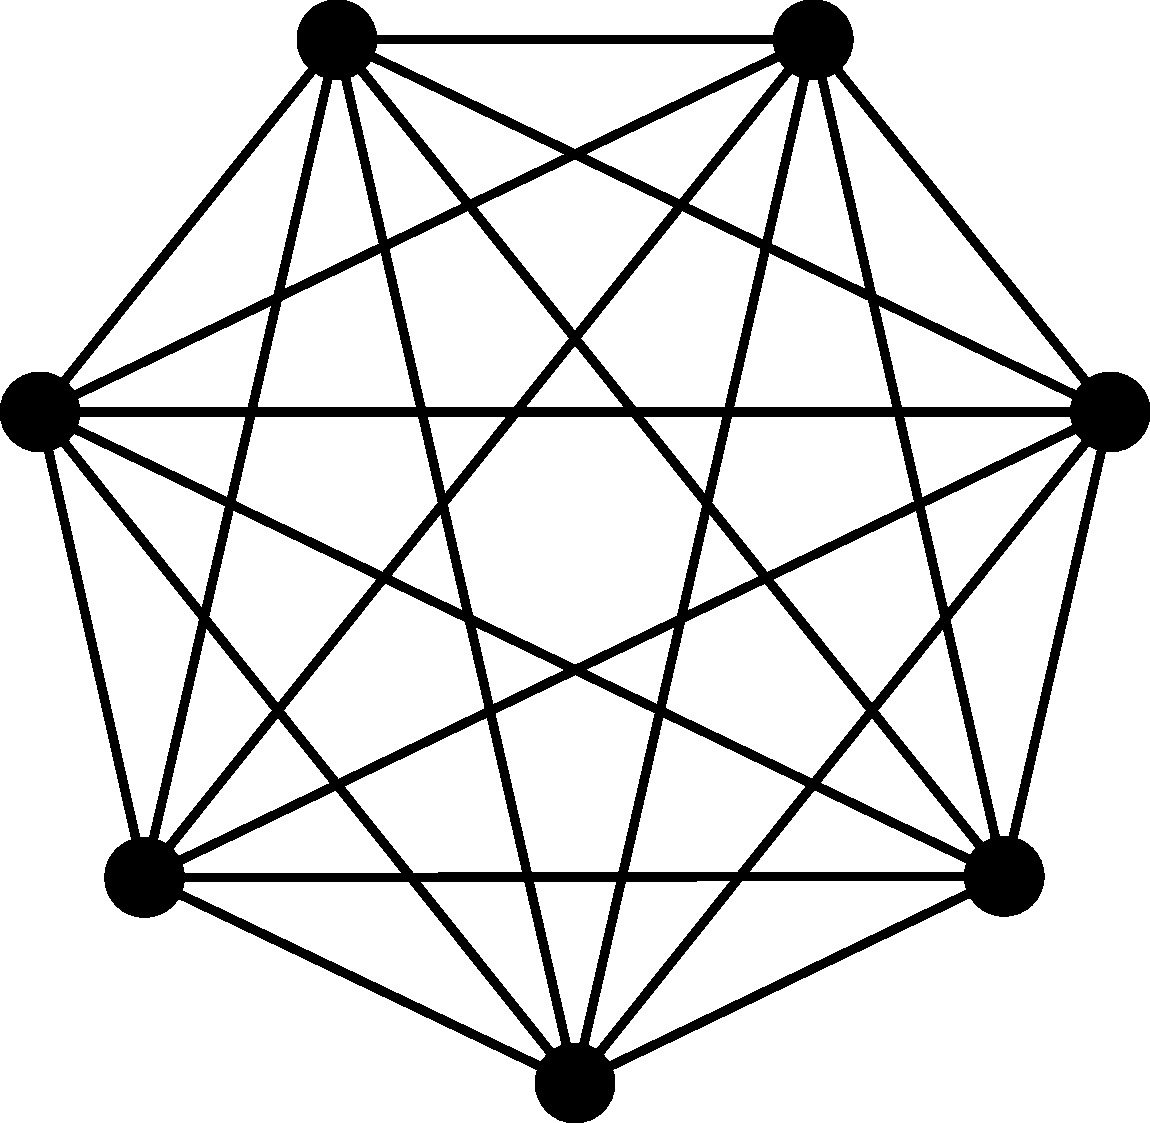
\includegraphics[scale=0.3]{3-4_binomial_distribution/figures/stars/dots_7_solution.pdf}
    \end{overprint}
\end{figure}

\onslide<2>\soln{\fbox{21}}
\end{frame} 



\begin{frame}
If there are 7 possible pizza toppings, and you will choose 3 of them, how many different pizzas are possible?
\pause
\begin{center}
\begin{tabular}{c c c c c}
CCCxxxx  & CxCxxCx  & CxxxxCC  & xCxCxxC  & xxCxCCx  \\
CCxCxxx  & CxCxxxC  & xCCCxxx  & xCxxCCx  & xxCxCxC  \\
CCxxCxx  & CxxCCxx  & xCCxCxx  & xCxxCxC  & xxCxxCC  \\
CCxxxCx  & CxxCxCx  & xCCxxCx  & xCxxxCC  & xxxCCCx  \\
CCxxxxC  & CxxCxxC  & xCCxxxC  & xxCCCxx  & xxxCCxC  \\
CxCCxxx  & CxxxCCx  & xCxCCxx  & xxCCxCx  & xxxCxCC  \\
CxCxCxx  & CxxxCxC  & xCxCxCx  & xxCCxxC  & xxxxCCC  
\end{tabular}
\end{center}
\pause
$${7\choose 3} = \frac{7!}{4! \cdot 3!} = \frac{7 \cdot 6 \cdot 5\cdot 4\cdot 3\cdot 2\cdot 1}{4\cdot 3\cdot 2\cdot 1\cdot 3\cdot 2\cdot 1} = \frac{7\cdot 6\cdot 5}{3\cdot2\cdot 1} = \pause \soln{\fbox{35}}$$

\pause
Notice, these rearrangements are like anagrams.

\end{frame} 




\begin{frame}
\frametitle{Combinatorics: combinations}
Combinations: list of all anagrams of a ``word" which contains only 2 letters. Often we use 1 for ``yes" or ``success" and use 0 for ``no'' or ``failure''.

\pause
for example: ~~0011 ~~0101 ~~0110 ~~1001 ~~1010 ~~1100

\vspace{10pt}
\pause
We define:
$$n = \text{word length}$$
$$r = \text{how many 1s}$$
The typical problem: We have $n$ objects and we will choose $r$ of them as ``yes"  (and the rest as ``no"). How many possibilities exist?
$$n\text{ choose } r = {}_nC_r = {n \choose r} = \frac{n!}{(n-r)! \cdot r!} $$
\end{frame}


\begin{frame}[fragile]
\frametitle{Evaluating $n$ choose $r$ with technology}
If we wanted to evaluate $40 \choose 27$...

Geogebra Scientific Calculator:
\begin{beamerboxesrounded}[shadow = true, lower = code body]{}
{
\begin{verbatim}
nCr(40, 27)
\end{verbatim}
}
\end{beamerboxesrounded}
    
R:
\begin{beamerboxesrounded}[shadow = true, lower = code body]{}
{
\begin{verbatim}
> choose(40,27)
[1] 12033222880
\end{verbatim}
}
\end{beamerboxesrounded}

TI Calculator:
\begin{beamerboxesrounded}[shadow = true, lower = code body]{}
{
\begin{verbatim}
40 nCr 27
\end{verbatim}
}
\end{beamerboxesrounded}

\end{frame}




%%%%%%%%%%%%%%%%%%%%%%%%%%%%%%%%%%%%%%%%%%%%%%%
\section{Binomial distribution}
%%%%%%%%%%%%%%%%%%%%%%%%%%%%%%%%%%%%%%%%%%%%%%%


\begin{frame}
Imagine a dice game where a 6 is ``success" and anything else is ``failure''. 

What is the probability of rolling 5 dice and getting 3 successes?
\pause

\vspace{40pt}
\solnGr{Well... first let's do something easier...}
\end{frame}



\begin{frame}
Imagine a dice game where a 6 is ``success" and anything else is ``failure''. 

What is the probability of rolling 5 dice and getting (in this order) success, fail, success, success, and fail.
$$P(10110) = \,?$$

\pause
\soln{$$P(10110) = \frac{1}{6} \cdot \frac{5}{6} \cdot \frac{1}{6} \cdot \frac{1}{6} \cdot \frac{5}{6} \approx 0.0032$$}

\pause \vfill
What is the probability of rolling 5 dice and getting (in this order) \\fail, fail, success, success, and success.
$$P(00111)=\,?$$

\pause
\soln{$$P(00111) = \frac{5}{6} \cdot \frac{5}{6} \cdot \frac{1}{6} \cdot \frac{1}{6} \cdot \frac{1}{6} \approx 0.0032 $$}

\vfill
\end{frame}



%%%%%%%%%%%%%%%%%%%%%%%%%%%%%%%%%%%%%%%%%%%%%%%%



\begin{frame}
Imagine a dice game where a 6 is ``success" and anything else is ``failure''. 

What is the probability of rolling 5 dice and getting 3 successes?
\pause

\soln{We need to consider how many (disjoint) ways we can accomplish 3 successes.} \pause
\begin{columns}
\begin{column}{0.6\textwidth}
\soln{
11100 ~ 11010 ~ 11001 ~ 10110 ~ 10101\\ 10011 ~ 01110 ~ 01101 ~ 01011 ~ 00111}
\end{column}
\begin{column}{0.3\textwidth}
\soln{
$${5 \choose 3} = 10 $$}
\end{column}
\end{columns}

\soln{
There are ten ways to get 3 successes from 5 trials.
\\\pause
Each way has an equal probability.
$$P(\text{a way}) = \left(\frac{1}{6}\right)^3 \left(\frac{5}{6}\right)^2 \approx 0.0032$$
\pause
Thus,
$$P(\text{3 successes}) = {\bf 10}\left(\frac{1}{6}\right)^3 \left(\frac{5}{6}\right)^2 \approx {\bf 0.032}$$
}
\end{frame}


\begin{frame}
\frametitle{Binomial mass function}
Let $X$ represent the number of successes when $n$ trials are performed and each trial has $p$ chance of success. We use a formula to calculate the probability that $X$ is $k$.

$$P(X=k) ~~~~{\LARGE \boldsymbol{=}}~~~~ {\Large \boldsymbol{{n \choose k}\, p^{k}(1-p)^{n-k}}} $$

For example, if $n=4$ and $p=0.1$, then:
\begin{tabular}{|c |c |c |}\hline
$k$ & $P(X=k)$ unsimped & $P(X=k)$ \\ \hline
0 & $(1)(0.1)^0(0.9)^4$ & 0.6561 \\
1 & $(4)(0.1)^1(0.9)^3$ & 0.2916 \\
2 & $(6)(0.1)^2(0.9)^2$ & 0.0486 \\
3 & $(4)(0.1)^3(0.9)^1$ & 0.0036 \\
4 & $(1)(0.1)^4(0.9)^0$ & 0.0001 \\ \hline
\end{tabular}

\end{frame}




\begin{frame}
\frametitle{Practice}
Find the probabilities of $X\sim Binomial(n=2,\,p=0.4)$.
\pause
\begin{center}\LARGE
\begin{tabular}{|c|c|c|} \hline
$k$ & $P(X=k)$ unsimplified & $P(X=k)$ simplified \\ \hline
\soln{0} & \soln{$(1)(0.4)^0(0.6)^2$} & \soln{0.36} \\
\soln{1} & \soln{$(2)(0.4)^1(0.6)^1$} & \soln{0.48} \\
\soln{2} & \soln{$(1)(0.4)^2(0.6)^0$} & \soln{0.16} \\\hline
\end{tabular}
\end{center}
\pause
Determine $P(X\ge 1)$. \pause
\soln{$$P(X\ge 1) = 0.64$$}
Determine the expected value. \pause
\soln{$$\mu = (0)(0.36) + (1)(0.48) + (2)(0.16) =\pause 0.8$$}
\end{frame}


\begin{frame}
\frametitle{Practice}
Let $X\sim Binomial(20,\,0.8)$. Calculate $P(X=15)$. \pause
\soln{$${20\choose 15}(0.8)^{15}(0.2)^{5} = \pause\fbox{0.1745595}$$}
\vfill
We are about to derive the following rules for binomials:
$$\mu = np$$
$$\sigma = \sqrt{np(1-p)}$$ 
Determine the expected value and standard deviation of $X$.\pause
\soln{$$\mu = (20)(0.8) = 16$$} \pause
\soln{$$\sigma = \sqrt{(20)(0.8)(0.2)} = 1.788854$$}
\vfill
\end{frame}


%%%%%%%%%%%%%%%%%%%%%%%%%%%%%%%%%%%%%%%%%%%%%%%
\section{A {\bf Binomial} is a sum of Bernoulli trials}
%%%%%%%%%%%%%%%%%%%%%%%%%%%%%%%%%%%%%%%%%%%%%%%


\begin{frame}
A Bernoulli trial is a random variable that can take on two possible values, 0 or 1, and has a $p$ chance of being 1.

\pause
Let $W\sim Bernoulli(p=0.6)$.
\begin{center}
\begin{tabular}{|c|c|}\hline
$w$ & $P(W=w)$ \\ \hline
0 & 0.4 \\
1 & 0.6 \\ \hline
\end{tabular}
\end{center}
Determine $\mu$ and $\sigma$.

\pause
\soln{$$\mu = (0)(0.4) + (1)(0.6) = 0.6$$
\\
$$\sigma = \sqrt{(0-0.6)^2(0.4) + (1-0.6)^2(0.6)} = 0.4899 $$
}
\end{frame}



\begin{frame}
Now, try this more generally. Let $W\sim Bernoulli(p)$. 

\pause
\begin{center}
\begin{tabular}{|c|c|}\hline
$w$ & $P(W=w)$ \\ \hline
0 & \soln{$(1-p)$} \\
1 & \soln{$p$} \\ \hline
\end{tabular}
\end{center}

\pause
Determine $\mu$ and $\sigma$.
\pause
\begin{align*}
\mu &= (0)(1-p) + (1)(p) = \fbox{p}\\\\
\sigma &= \sqrt{(0-p)^2(1-p) + (1-p)^2p} \\
&=\sqrt{p^2(1-p) + (1-p)^2p} \\
&=\sqrt{p^2-p^3 + p-2p^2+p^3} \\
&=\sqrt{p-p^2} \\
&=\sqrt{p(1-p)}
\end{align*}
\end{frame}



\begin{frame}
\frametitle{A binomial is a sum of Bernoulli trials}
In chapter 2.4 we learned the following rules.
$$E(W_1 + W_2 + \cdots + W_n) = E(W_1) + E(W_2) + \cdots + E(W_n) $$
$$Var(W_1 + W_2 + \cdots + W_n) = Var(W_1) + Var(W_2) + \cdots + Var(W_n) $$
\pause
For a specific $p$, for all $i$ between 1 and $n$, let $W_i\sim Bernoulli(p)$. Let $X$ represent the sum of those variables, making $X\sim Binomial(n,p)$.
$$X = \sum_{i=1}^n W_i $$

If so, then we know (by using those rules):
$$E(X) = np $$
$$Var(X) = np(1-p) $$
$$SD(X) = \sqrt{np(1-p)} $$
\end{frame}



\begin{frame}
\frametitle{Binomial mean and standard deviation}
Let $X\sim Binomial(n,p)$.
The mean (expected value) of a binomial distribution:
{\LARGE $$\mu = np $$}
The standard deviation of a binomial distribution:
{\LARGE $$ \sigma = \sqrt{np(1-p)} $$}
\end{frame}


\section{Binomial Distributions are (often) approximately normal}

\begin{frame}
\frametitle{Binomial Distributions are (often) approximately normal}
Let $X\sim Binomial(n=20,\,p=0.7)$, which has $\mu = 14$ and $\sigma = 2.05$. \pause

Let $Y\sim N(\mu=14,\, \sigma=2.05)$. \pause

Let's overlay two density functions: the discrete binomial function and the continuous normal function. \pause
\begin{center}
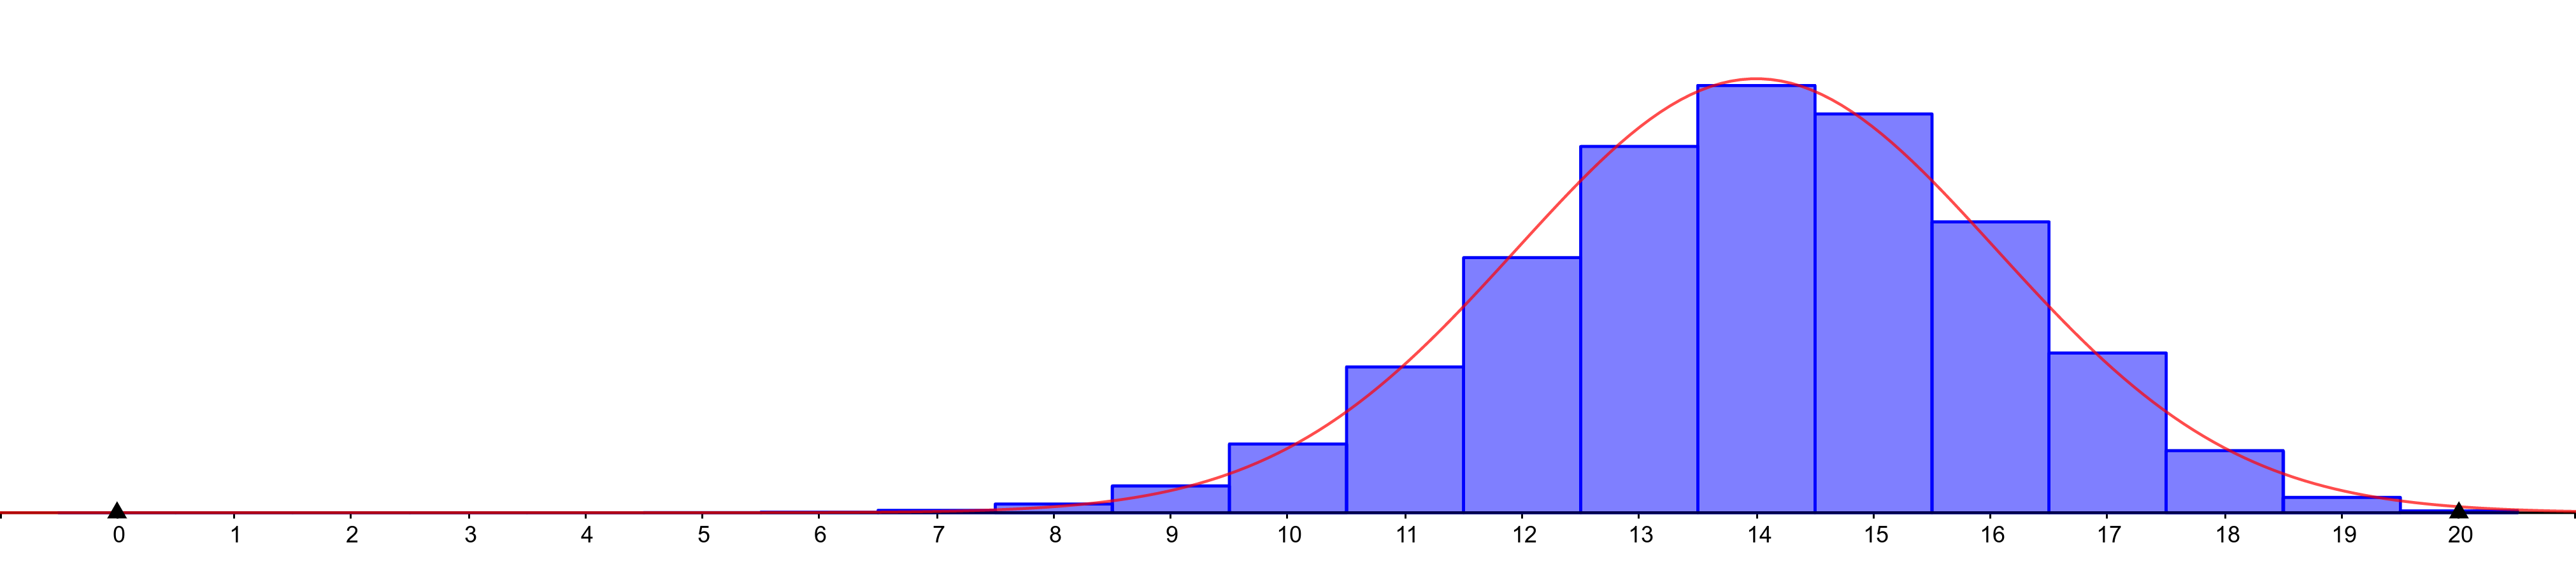
\includegraphics[scale=0.08]{3-4_binomial_distribution/figures/bin_norm/geogebra-export.png}
\end{center}

Rule of thumb:\\
If $np \ge 10$ and $n(1-p) \ge 10$, then the normal approximation will work well (except in the tails).
\end{frame}


\begin{frame}
\frametitle{Practice}
Let $X\sim Binomial(n=20,\,p=0.7)$, which has $\mu = 14$ and $\sigma = 2.05$. \pause

Let $Y\sim N(\mu=14,\, \sigma=1.79)$. \pause

Estimate $P(12 \le X \le 16)$ using the normal approximation.
\begin{center}
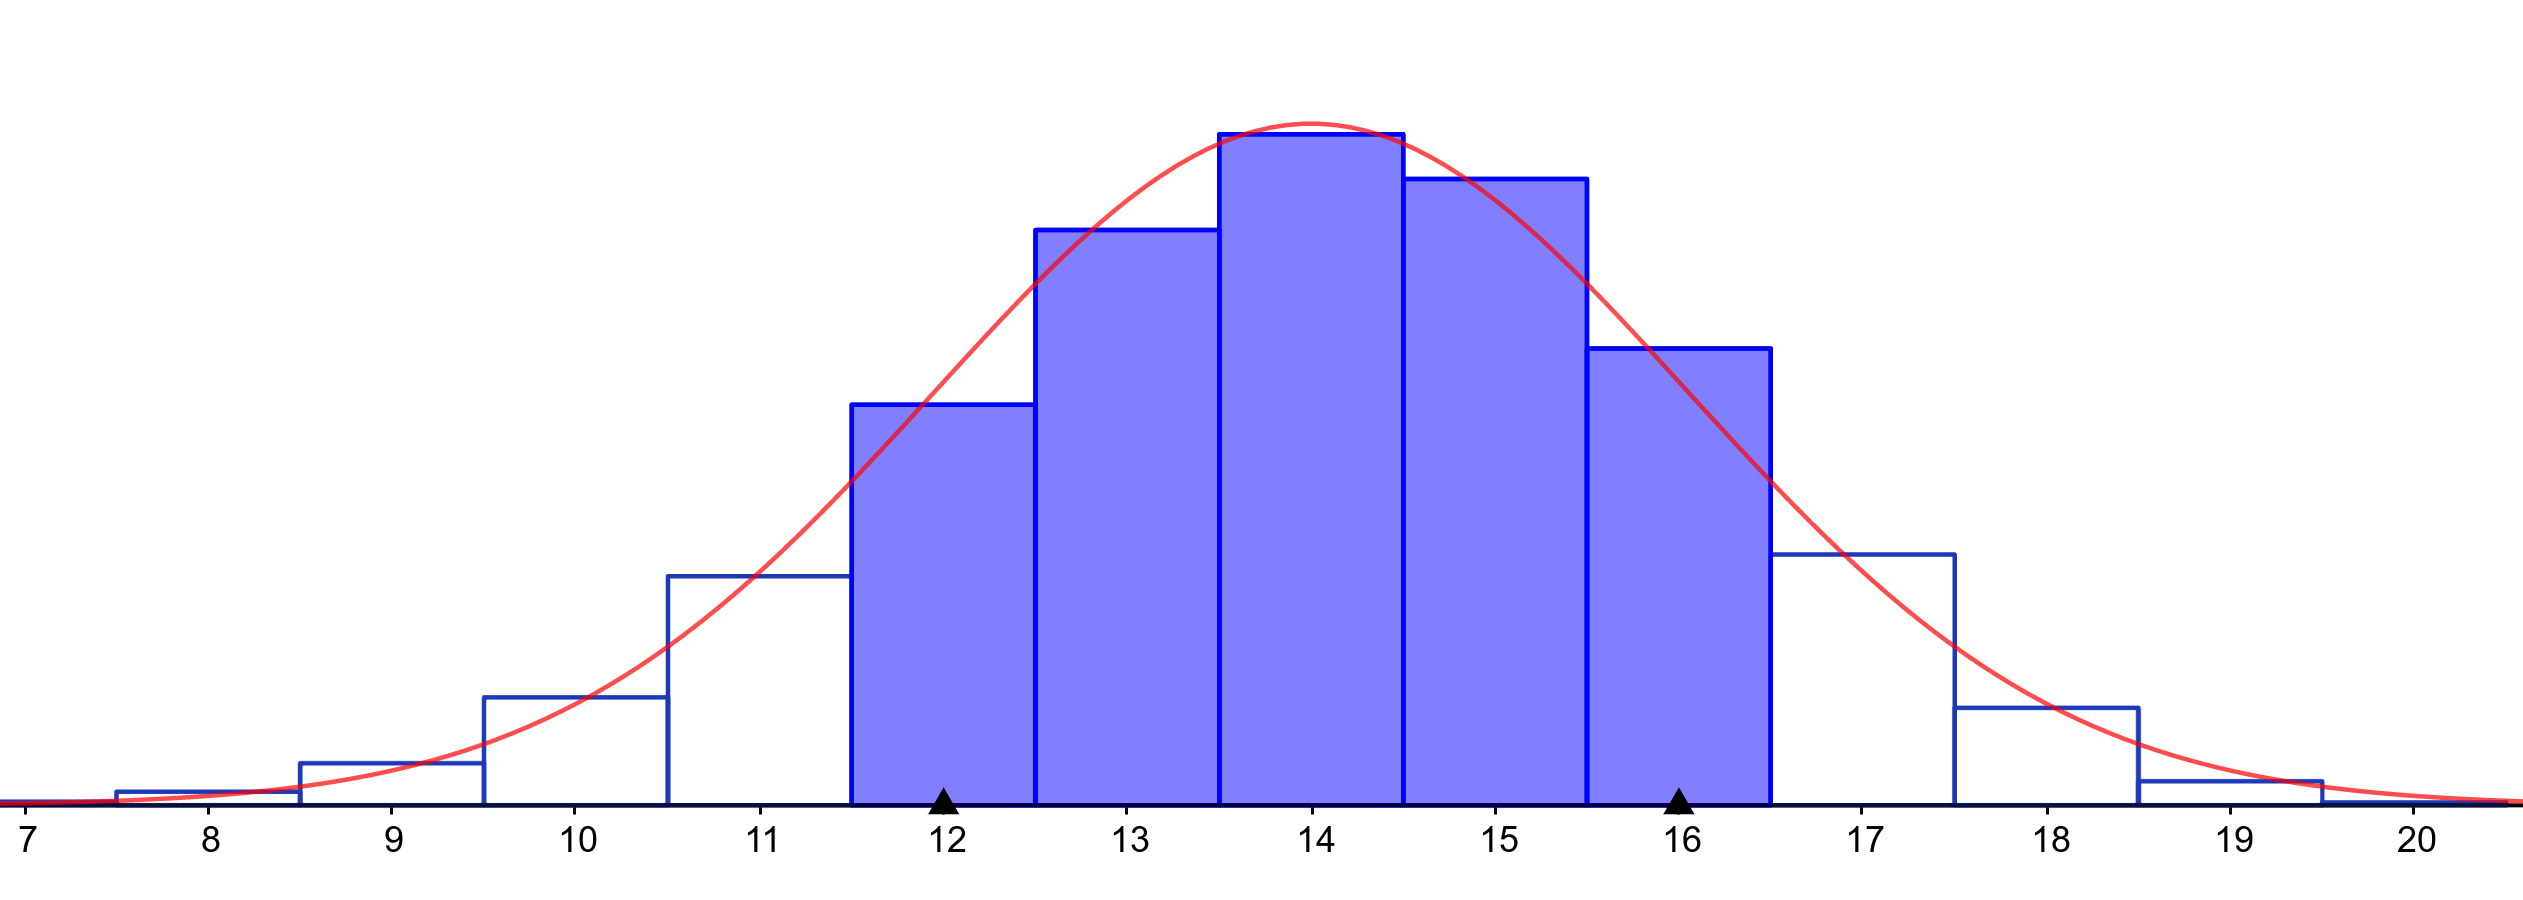
\includegraphics[scale=0.08]{3-4_binomial_distribution/figures/bin_norm/geogebra-export2.png}
\end{center}
\pause
\soln{$$P(12 \le X \le 16) \approx P(11.5 < Y < 16.5)$$}
\pause
\soln{$z_1 = \frac{11.5-14}{2.05} = -1.22$}~~\pause~~
\soln{$z_2 = \frac{16.5-14}{2.05} =  1.22$}\pause
\soln{$$P(12 \le X \le 16) \approx \Phi(1.22)-\Phi(-1.22) = \fbox{0.78}$$}

\end{frame}






\end{document}
